\documentclass[a4paper]{article}

\usepackage{fullpage} % Package to use full page
\usepackage{parskip} % Package to tweak paragraph skipping
\usepackage{tikz} % Package for drawing
\usepackage{amsmath}
\usepackage{hyperref}
\usepackage{amssymb}
\usepackage{tikz-qtree}
\usepackage{amsthm}

\usepackage{tkz-graph}

%https://tex.stackexchange.com/questions/229355/algorithm-algorithmic-algorithmicx-algorithm2e-algpseudocode-confused
\usepackage{algorithm}
\usepackage{algorithmicx}
\usepackage{algpseudocode}

\usepackage{graphicx}
\graphicspath{ {./resources/} }

%https://tex.stackexchange.com/questions/165021/fixing-the-location-of-the-appearance-in-algorithmicx-environment
\usepackage{float}% http://ctan.org/pkg/float

%https://tex.stackexchange.com/questions/25369/how-to-rotate-a-table
\usepackage[graphicx]{realboxes}
\title{23 Minimum Spanning Trees}
\author{Ling Tan}
\date{2018-10}

\begin{document}
%\maketitle

\textcolor{red}{\textit{mst}} denotes minimum spanning tree
\section*{23.1 Growing a minimum spanning tree}
\textcolor{blue}{Definition}: A \textbf{\textit{cut}} in $G=(V,E)$ is a partition of $V$ such that $V=V_1\cup V_2, V_1\cap V_2=\emptyset$. \\
\\
\textcolor{blue}{Definition}: A \textbf{\textit{crossing}} edge connects a vertex in $V_1$ with a vertex in $V_2$.\\
\\
\textcolor{blue}{Property}: Every minimum crossing edge $\in$ some mst of $G$, and every mst contains a minimum crossing edge.\\
Proof: by contradiction\\
Assume that $e_1$, the minimum crossing edge, does not belong to any mst. Consider a minimum $T$ of $G$. Then $T$ contains one of the crossings edges $e_1,e_2,\ldots, e_k$ (if no then $T$ is a forest, not a tree). Assume $e_i\in T$, construct another $T'=T \backslash \{e_1\}\cup \{e_i\}$.
\begin{align*}
W(T')&=W(T)-W(e_i)+W(e_1)\\
&= W(T)-\big(W(e_i)-W(e_1)\big)\\
&\leq W(T) \\
&W(T')<W(T)\text{ is impossible}\\
\Rightarrow &W(T')=W(T)\\
\text{Contradiction}&\text{: since $T'$ contains $e_1$, and is also a mst.} 
\end{align*}

\section*{23.2 The algorithms of Kruskal and Prim}

\subsection*{Prim-Jarnik algorithm}
The set of edges selected for the minimum spanning tree forms a subtree of the graph.
\begin{enumerate}
    \item Start with an arbitrary vertex and grow it an edge at a time until a spanning tree is obtained.
    \item At each step a vertex $u$ not in the tree, connected by the smallest possible cost edge to the subtree already built, is added.
    \item By the theorem, this creates a minimum spanning tree.
\end{enumerate}

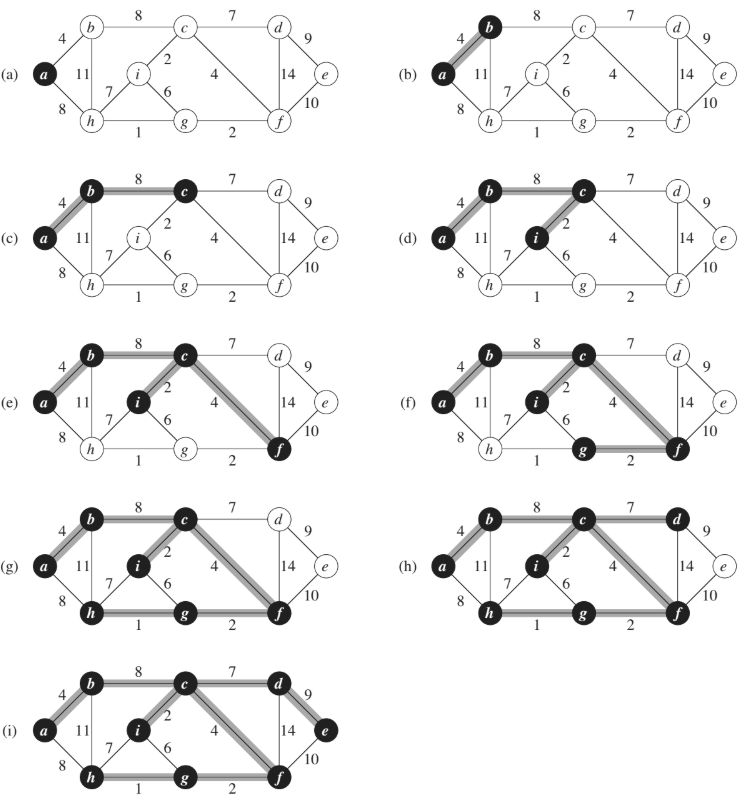
\includegraphics[width=\textwidth]{Prim}

\subsection*{Kruskal's algorithm}
\begin{enumerate}
    \item Sort the edges of $G$ as follows:\\
    $W(e_1)\leq W(e_2)\leq \cdots \leq W(e_m)$
    \item Construct a mst $T$ as follows:\\
    add $e_1\in T$\\
    add $e_2\in T$\\
    keep adding an edge $e_i, i=3,4,\cdots, m$\\
    \hspace*{1em}if current $T\cup \{e_i\}$ does not contain a cycle than add $e_i\in T, T={e_1,e_2,\ldots, e_i}$\\
    \hspace*{1em}if $T$ has $n-1$ edges, stop, then $T$ is mst.
\end{enumerate}
Complexity:
\begin{enumerate}
    \item step1 merge sort: $O(|E|\log{|E|})$
    \item step2 $O(|E|)$
    \item total:
        \begin{align*}
            O(|E|\log{|E|})+O(|E|)&=O(|E|\log{|E|})\\
            &=O(|V|^2\log{|V|})
        \end{align*}
\end{enumerate}
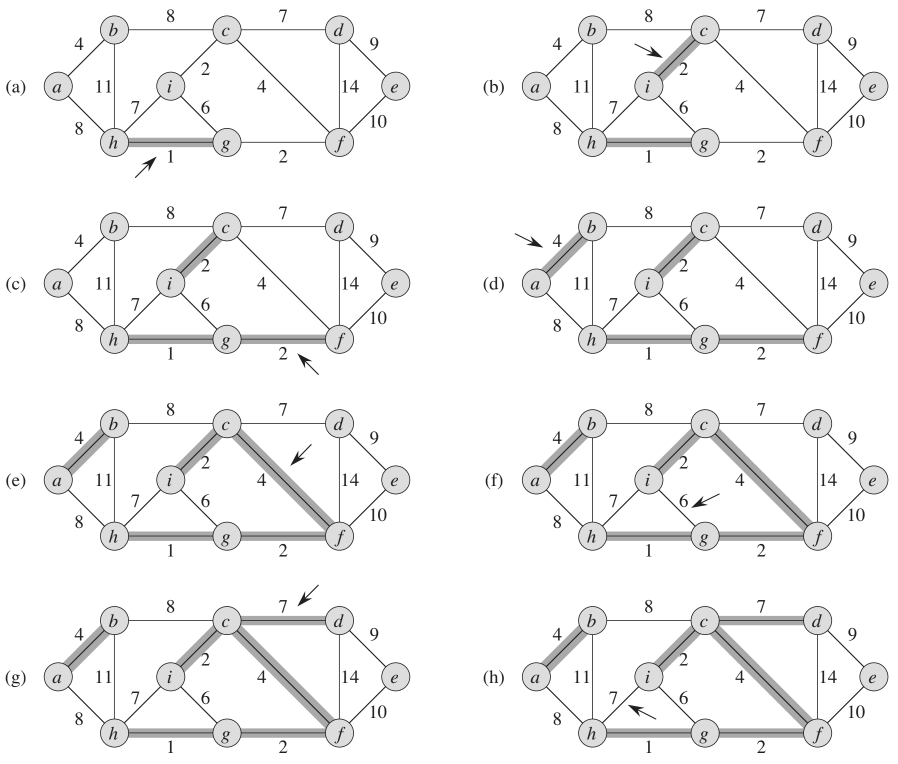
\includegraphics[width=\textwidth]{Kruskal1}
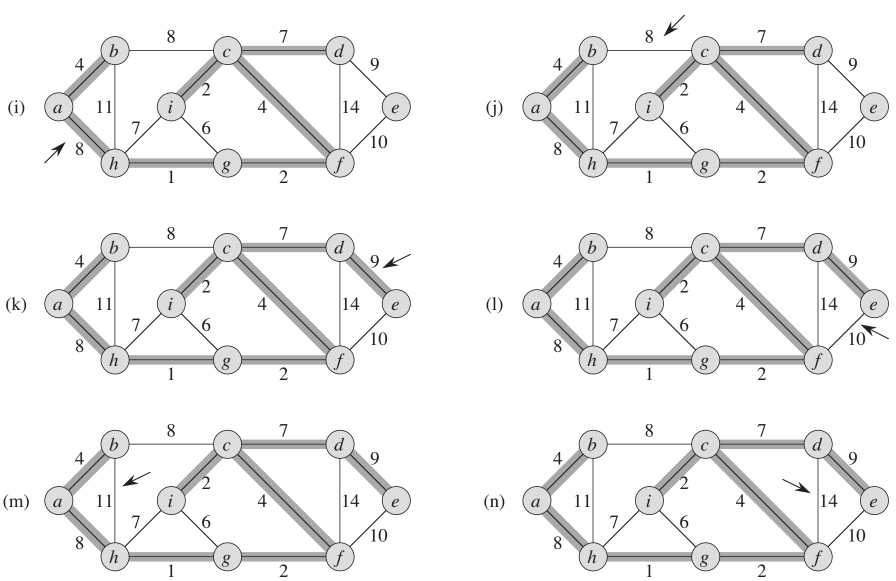
\includegraphics[width=\textwidth]{Kruskal2}
\subsection*{Greedy Choice property}
$\exists{mst}$ of $G=(V,E)$ that includes edge $e_1$, where $W(e_1)\leq W(e_2)\leq \cdots W(e_m)$.
\begin{proof}
Consider a mst $T$. \\
\begin{center}
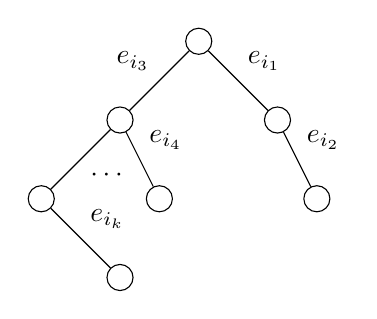
\begin{tikzpicture}[auto]
   \begin{scope}[every node/.style={circle,draw=black}]
    \node (v1) at (0,0) {};
    \node (v2) at (-1,-1) {};
    \node (v3) at (-2,-2) {};
    \node (v4) at (-1,-3) {};
    \node (v5) at (-0.5,-2) {};
    \node (v6) at (1,-1) {};
    \node (v7) at (1.5,-2) {};
   \end{scope}
   \begin{scope}[every edge/.style={draw=black}]
    \draw  (v2) edge node{$e_{i_3}$} (v1);
    \draw  (v2) edge node{$\cdots$} (v3);
    \draw  (v2) edge node{$e_{i_4}$} (v5);
    \draw  (v3) edge node{$e_{i_k}$} (v4);
    \draw  (v1) edge node{$e_{i_1}$} (v6);
    \draw  (v6) edge node{$e_{i_2}$} (v7);
   \end{scope}
\end{tikzpicture}
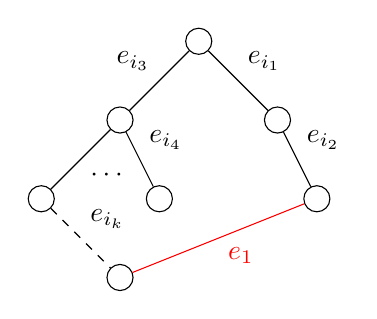
\begin{tikzpicture}[auto]
   \begin{scope}[every node/.style={circle,draw=black}]
    \node (v1) at (0,0) {};
    \node (v2) at (-1,-1) {};
    \node (v3) at (-2,-2) {};
    \node (v4) at (-1,-3) {};
    \node (v5) at (-0.5,-2) {};
    \node (v6) at (1,-1) {};
    \node (v7) at (1.5,-2) {};
   \end{scope}
   \begin{scope}[every edge/.style={draw=black}]
    \draw  (v2) edge node{$e_{i_3}$} (v1);
    \draw  (v2) edge node{$\cdots$} (v3);
    \draw  (v2) edge node{$e_{i_4}$} (v5);
    \draw  (v3) [dashed] edge node{$e_{i_k}$} (v4);
    \draw  (v1) edge node{$e_{i_1}$} (v6);
    \draw  (v6) edge node{$e_{i_2}$} (v7);
    \draw  (v7) edge[red] node{$e_{1}$} (v4);
   \end{scope}
\end{tikzpicture}
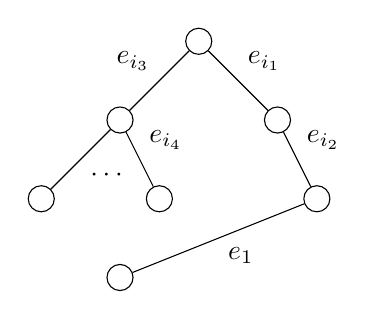
\begin{tikzpicture}[auto]
   \begin{scope}[every node/.style={circle,draw=black}]
    \node (v1) at (0,0) {};
    \node (v2) at (-1,-1) {};
    \node (v3) at (-2,-2) {};
    \node (v4) at (-1,-3) {};
    \node (v5) at (-0.5,-2) {};
    \node (v6) at (1,-1) {};
    \node (v7) at (1.5,-2) {};
   \end{scope}
   \begin{scope}[every edge/.style={draw=black}]
    \draw  (v2) edge node{$e_{i_3}$} (v1);
    \draw  (v2) edge node{$\cdots$} (v3);
    \draw  (v2) edge node{$e_{i_4}$} (v5);
    \draw  (v1) edge node{$e_{i_1}$} (v6);
    \draw  (v6) edge node{$e_{i_2}$} (v7);
    \draw  (v7) edge node{$e_{1}$} (v4);
   \end{scope}
\end{tikzpicture}
\end{center}
If $e_1\in T$, then done. \\
If $e_1\notin T$, then consider $T\cup \{e_1\}$ which will contain a single cycle, say with edges $e_1,e_{i_1},e_{i_2},\cdots, e_{i_k}$ where $W(e_1)\leq W(e_{i_1})\leq W(e_{i_2})\leq \cdots W(e_{i_k})$. Delete edge $e_{i_k}$ from $T\cup \{e_1\}$ to obtain tree $T'=T\cup \{e_1\}\backslash \{e_{i_k}\}$. $W(T')=W(T)+W(e_1)-W(e_{i_k})\leq W(T)$.
Since $T$ is a mst, then $W(T')< W(T)$ is not possible. Thus, $W(T')=W(T)\Rightarrow T'$ is a mst.
\end{proof}
\subsection*{Optimal Substructure property}
Assume that $T$ is a mst of $G$. Consider the edges of $T$, where $W(e_1)\leq W(e_2)\leq \cdots W(e_m)$. Remove $e_1(u,v)$, $T$ would split into 2 sub-trees, say $T_u=(V_u,E_u)$ and $T_v=(V_v,E_v)$. $T_u$ is a sub-tree generate by $u$, meaning that connected to $u$ by a unique path; and same to $T_v$. Then, consider $G_u=(V_u,{E_u}')\subseteq G$ generated by the vertices of $V_u$; the same with $G_v=(V_v,{E_v}')\subseteq G$. Then $T_u$ is a mst of $G_u$, and $T_v$ for $G_v$.
\begin{proof}
Consider a mst of $G_u$, call it $T_1$, then $W(T_1)\leq W(T_u)$. Same way, say $T_2$ is a mst of $G_v$, then $W(T_2)\leq W(T_v)$. Consider min weight crossing edge $e=\{v_u,v_v\}$, and another crossing edge $e_k$, then $W(T_1\cup T_2\cup e)$ is a spanning tree of $G$ such that
\begin{align*}
    W(T_1\cup T_2\cup e)&=W(T_1)+W(T_2)+W(e)\\
    &\leq W(T_u)+W(T_v)+W(e_k)\\
    &=W(T)\\
    \Rightarrow&T_1\cup T_2\cup e \text{ is a mst,}& W(T)\text{ is mst}\\
    &\text{ and }W(T_1)=W(T_u),W(T_2)=W(T_v),W(e)=W(e_k)
\end{align*}
\end{proof}
\end{document}